% !TEX root = ./cvl.tex
\section{CVL algorithm}

The clauses of the CVL language were introduced in Section~\ref{sec:language}. In this section we describe how the various clauses are transformed into an execution plan. CVL is compiled to a specific engine for execution, and there are in principle many types of plans. In this work we consider only one type of plan, namely the \emph{bottom-up} plan. A high-level view of compiling CVL to a bottom-up plan is shown in Figure~\ref{fig:compilation}.

\begin{figure}[htbp]
\begin{center}
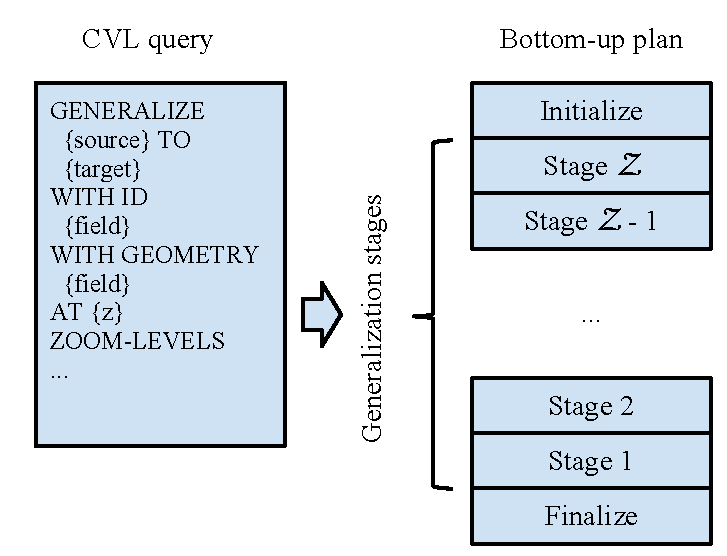
\includegraphics[scale=.75]{figs/cvl_compilation.pdf}
\caption{Compiling CVL to a bottom-up plan}
\label{fig:compilation}
\end{center}
\end{figure}

The bottom-up plan consists of three overall phases. A \emph{initialization} phase, a \emph{generalization} phase, and an \emph{finalization} stage. During the initializes phase the elements of the input are ranked and partitioned according to the CVL clauses for ranking and partitioning. The generalization phase consists a $\mathcal{Z}$ stages are executed separately (e.g. in parallel) for each partition. The output of stage $i$ is used as input to stage $i+1$. The bottom-up plan generalizes the dataset starting with the highest scale, and ending with the lowest scale. Intuitively, the records that survive the generalization process at stage $i$ (corresponding to some zoom-level $z$), are copied to stage $i+1$ (corresponding to some zoom-level $z-1$).

A single stage in the generalization phase consists of five sub-stages, shown in Figure~\ref{fig:stages}.

 the $\mathcal{Z}$ stages   of the elements in the input. The output of one stage is used as input to the next stage. Inside 


used by the CVL algorithm to produce a generalized dataset. See Figure~\ref{fig:evaluation} for a top down view of the algorithm performed by CVL.

\begin{figure}[htbp]
\begin{center}
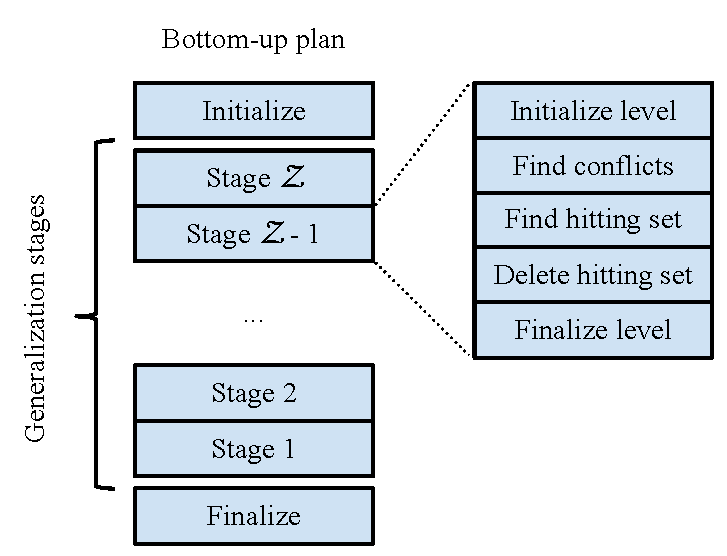
\includegraphics[scale=.75]{figs/cvl_stages.pdf}
\caption{Stages of the bottom-up plan}
\label{fig:stages}
\end{center}
\end{figure}

Each record $r \in O$ correponds to a record $r' \in I$, and for each record $r' \in I$ there may be up to $\mathcal{Z}$ records in $O$ representing it at different scales. To make things easier to explain we consider these records to be logically the same record.

For each record $r \in I$, the record is either represented at zoom-level $z$ or it has been deleted at a higher zoom-level $z': z < z' < \mathcal{Z}$.

A property of the algorithm is that the records stored for a zoom-level $z$ are a subset of the records stored at zoom-level $z+1$. This means that the \emph{zoom-consistency} constraint~\cite{fusiontables} is automatically enforced by the algorithm.

The CVL algorithm computes the zoom-levels in reverse order, i.e. by $z = \mathcal{Z}-1, \dots, 0$. At each zoom-level there are two main task performed by the CVL algorithm: \emph{finding conflicts} and \emph{resolving conflicts}. Before we can talk about conflicts, we need to define cartographic constraints in the context of CVL, as the notion of a conflict depends upon this definition.

\subsection{Cartographic constraints in CVL}

In CVL a cartographic constraint is a condition that must hold for all record subsets of a given size. Constraints are evaluated separately for different partitions and repeatedly at each zoom-level.

We formally consider the following two constraints in our work, but note that with our implementation of CVL it is easy to define new constraints. 

\begin{description}
\item [Proximity] Any two records must separated by at least $d$ pixels
\item [Visibility] Given a uniform grid of cells at most $K$ records may intersect any given cell
\end{description}

\subsection{Conflicts and hitting sets}

Given this brief introduction to constraints, we can now introduce the notion of a conflict. 
A conflict is a record subset for which a given constraint does not hold. As constraints are formulated for record subsets of a given size, it follows that a conflict can be resolved by deleting some of the records in the conflict from the current zoom-level.


\subsection{Cartographic constraints and conflicts}

We use two related terms to deal with selection of records at multiple zoom-levels: Constraints and conflicts. A \emph{constraint} states a condition that must hold over a set of records. A \emph{conflict} represents a subset of records that together violate a constraint. A conflict can always be resolved by deleting some of the records, indicated by the \emph{degree} of the conflict.

\subsubsection{Example}
Consider a proximity constraint that states that every pair of records must be separated by some minimum distance. Evaluating this constraint over a set of records produces a conflict for each a pair of records that are too close together. For each conflict, one of the records must be deleted in order to respect the constraint.

\subsection{Constraints}






%%%%%%
\section{Algorithm}

\subsection{K-Hitting Set Problem}

\subsubsection{Modelling as Hitting Set Problem}


\subsubsection{Algorithm for K-Hitting Set Problem}

One way to solve the problem is to transform the K-hitting sets problem to a normal hitting set problem. This can be done by breaking up a every conflict set with $minhits=n>1$ into $k+n \choose k+1$ distinct subsets. At this point we can use the set cover approximation algorithm on resulting conflict sets.

Instead of modifying the conflict sets to get a hitting set problem, we can modify the algorithm for hitting set (in the obvious way). Can we prove the same bound?

\subsection{Bottom-up algorithm}

\subsubsection{Initialization step}

\subsubsection{Analysis step}

Find all conflicts for constraint.

\subsubsection{Modification step}

Initialize level Z. Delete record from level, copy level to next level, simplify record.

\subsubsection{Postprocessing}

Simplification


\subsection{Approximation bound based on exponential reduction}